\documentclass[conference]{IEEEtran}
\IEEEoverridecommandlockouts
% The preceding line is only needed to identify funding in the first footnote. If that is unneeded, please comment it out.
\usepackage{cite}
\usepackage{amsmath,amssymb,amsfonts}
\usepackage{algorithmic}
\usepackage{graphicx}
\usepackage{textcomp}
\usepackage{xcolor}
\usepackage{subcaption}
\def\BibTeX{{\rm B\kern-.05em{\sc i\kern-.025em b}\kern-.08em
    T\kern-.1667em\lower.7ex\hbox{E}\kern-.125emX}}
\begin{document}

\title{Implement of Pilotnet on Caffe deeplearning framework\\
{\footnotesize \textsuperscript}
\thanks{Identify applicable funding agency here. If none, delete this.}
}

\author{\IEEEauthorblockN{1\textsuperscript{st} Ruzhuo Wang}
\IEEEauthorblockA{\textit{University of California, Riverside} \\
\textit{Riverside, California}\\
rwang085@ucr.edu}

}

\maketitle

\begin{abstract}
   In the target paper~\cite{b1}, they trained a Convolutional Neural Network (CNN) to map raw pixels from a single front-facing camera directly to steering commands. Their result is said to be 98\% autonomy value for a typical drive in Monmouth County NJ from their office in Holmdel to Atlantic Highlands.\par
   So I want to find out how they achieve that much high autonomy value, since the target paper do not provide any source code or their training dataset, so I build the exact architecture of Pilotnet as is mentioned in the targeted paper, and the driving dataset is captured from the front camera on a driving vehicle. 
\end{abstract}

\begin{IEEEkeywords}
Convolutional neural Network, Pilotnet, Caffe~\cite{b4}
\end{IEEEkeywords}

\section{Introduction}
CNNs have revolutionized pattern recognition. Prior to the widespread adoption of CNNs, most pattern recognition tasks were performed using an initial stage of hand-crafted feature extraction followed by a classifier. The breakthrough of CNNs is that features are learned automatically from training examples. The CNN approach is especially powerful in image recognition tasks because the convolution operation captures the 2D nature of images. Also, by using the convolution kernels to scan an entire image, relatively few parameters need to be learned compared to the total number of operations.\par
In this project, I search the Internet and find a driving dataset that is captured from the front camera on a driving vehicle, then I build the exact architecture of Pilotnet on the Caffe deep learning framework, modified the parameters and trained the network.
\subsection{End to End deep learning}
End to end (E2E)~\cite{b2} deep learning is the idea of instead of engineering a lot of presentations, you can output more complex things.\par


\subsection{Convolutional Neural Network}
In deep learning, a convolutional neural network (CNN, or ConvNet) is a class of deep neural networks, most commonly applied to analyzing visual imagery.\par

CNNs use a variation of multilayer perceptrons designed to require minimal preprocessing. They are also known as shift invariant or space invariant artificial neural networks (SIANN), based on their shared-weights architecture and translation invariance characteristics.\par

Convolutional networks were inspired by biological processes in that the connectivity pattern between neurons resembles the organization of the animal visual cortex. Individual cortical neurons respond to stimuli only in a restricted region of the visual field known as the receptive field. The receptive fields of different neurons partially overlap such that they cover the entire visual field.\par

CNNs use relatively little pre-processing compared to other image classification algorithms. This means that the network learns the filters that in traditional algorithms were hand-engineered. This independence from prior knowledge and human effort in feature design is a major advantage.\par

They have applications in image and video recognition, recommender systems, image classification, medical image analysis, and natural language processing.
~\cite{b5}

\section{Caffe}
Caffe is a deep learning framework made with expression, speed, and modularity in mind. It is developed by Berkeley AI Research (BAIR) and by community contributors. Yangqing Jia created the project during his PhD at UC Berkeley. Caffe is released under the BSD 2-Clause license.

\begin{itemize}
	\item Expressive architecture encourages application and innovation. Models and optimization are defined by configuration without hard-coding. Switch between CPU and GPU by setting a single flag to train on a GPU machine then deploy to commodity clusters or mobile devices.
	\item Extensible code fosters active development. In Caffe’s first year, it has been forked by over 1,000 developers and had many significant changes contributed back. Thanks to these contributors the framework tracks the state-of-the-art in both code and models.
	\item Speed makes Caffe perfect for research experiments and industry deployment. Caffe can process over 60M images per day with a single NVIDIA K40 GPU*. That’s 1 ms/image for inference and 4 ms/image for learning and more recent library versions and hardware are faster still. We believe that Caffe is among the fastest convnet implementations available.
	\item Community: Caffe already powers academic research projects, startup prototypes, and even large-scale industrial applications in vision, speech, and multimedia. Join our community of brewers on the caffe-users group and Github.
	
\end{itemize}


\subsection{Pilotnet}
They trained a convolutional neural network (CNN) to map raw pixels from a sin-
gle front-facing camera directly to steering commands. This end-to-end approach
proved surprisingly powerful. With minimum training data from humans the system learns to drive in traffic on local roads with or without lane markings and on
highways. It also operates in areas with unclear visual guidance such as in parking
lots and on unpaved roads.\par
The system automatically learns internal representations of the necessary processing steps such as detecting useful road features with only the human steering angle
as the training signal. We never explicitly trained it to detect, for example, the outline of roads.\par
Compared to explicit decomposition of the problem, such as lane marking detection, path planning, and control, our end-to-end system optimizes all processing
steps simultaneously. We argue that this will eventually lead to better performance and smaller systems. Better performance will result because the internal
components self-optimize to maximize overall system performance, instead of optimizing human-selected intermediate criteria, e. g., lane detection. Such criteria
understandably are selected for ease of human interpretation which doesn’t automatically guarantee maximum system performance. Smaller networks are possible because the system learns to solve the problem with the minimal number of processing steps.\par
We used an NVIDIA DevBox and Torch 7 for training and an NVIDIA
DRIVE TM PX self-driving car computer also running Torch 7 for determining
where to drive. The system operates at 30 frames per second (FPS).

\section{System framework}

\subsection{Data preparation}
I write a python script(datasetreader.py) to divide the dataset into two parts, 7/8 of the driving dataset has been treat as training dataset, the other 1/8 of the driving dataset has been treat as test dataset, the driving dataset is consist of 45406 images that captured from a front camera on a driving car. I download this dataset from SullyChen's github repository~\cite{b3}.

\begin{figure}[h]
	\begin{center}		
		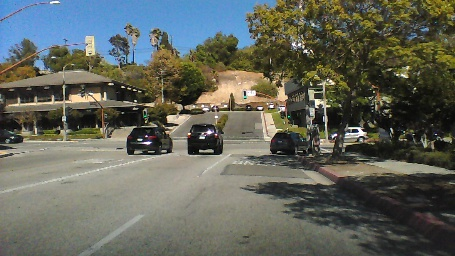
\includegraphics[width=0.8\linewidth]{fig1.jpg}
	\end{center}
	\caption{Example of an image from testing dataset}
	\label{fig:long1}
\end{figure}

\subsection{Pilotnet architecture}

The original network consists of 9 layers, including a normalization layer, 5 convolutional layers and 3 fully connected layers. In the target paper, they use strided convolutions in the first three convolutional layers with a $2\times 2$ stride and a $5\times 5$ kernel and a non-strided convolution with a $3\times 3$ kernel size in the last two convolutional layers.

\begin{figure}[h]
	\begin{center}		
		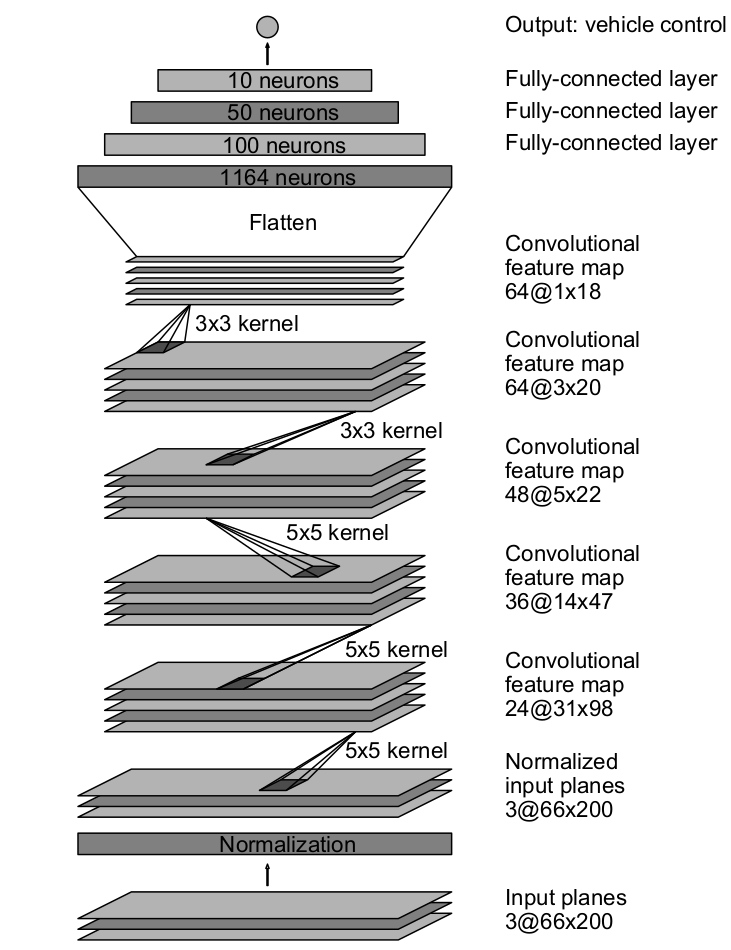
\includegraphics[width=0.8\linewidth]{fig2.png}
	\end{center}
	\caption{Pilotnet architecture}
	\label{fig:long2}
\end{figure}


\subsection{Important preparation before training}


Because the Pilotnet is an end to end network, so it require labeled dataset as training and testing dataset, and for Caffe deeplearning frame work, in order to convert the steering angle into lmdb format, the steering angle should be converted to positive integers. So I write a python script(label.py) to transfer the steering angle from float number into 0 to 36 positive integers, because the steering angle is similar to a Gaussian distribution, the majority steering angle is around 0, so I map the steering angle with the value within -140 to 140 into 1 to 35, the steering angle with the value less than -140 into 0, the steering angle with the value bigger than 140 into 36.


\begin{figure}[h]
	\begin{center}		
		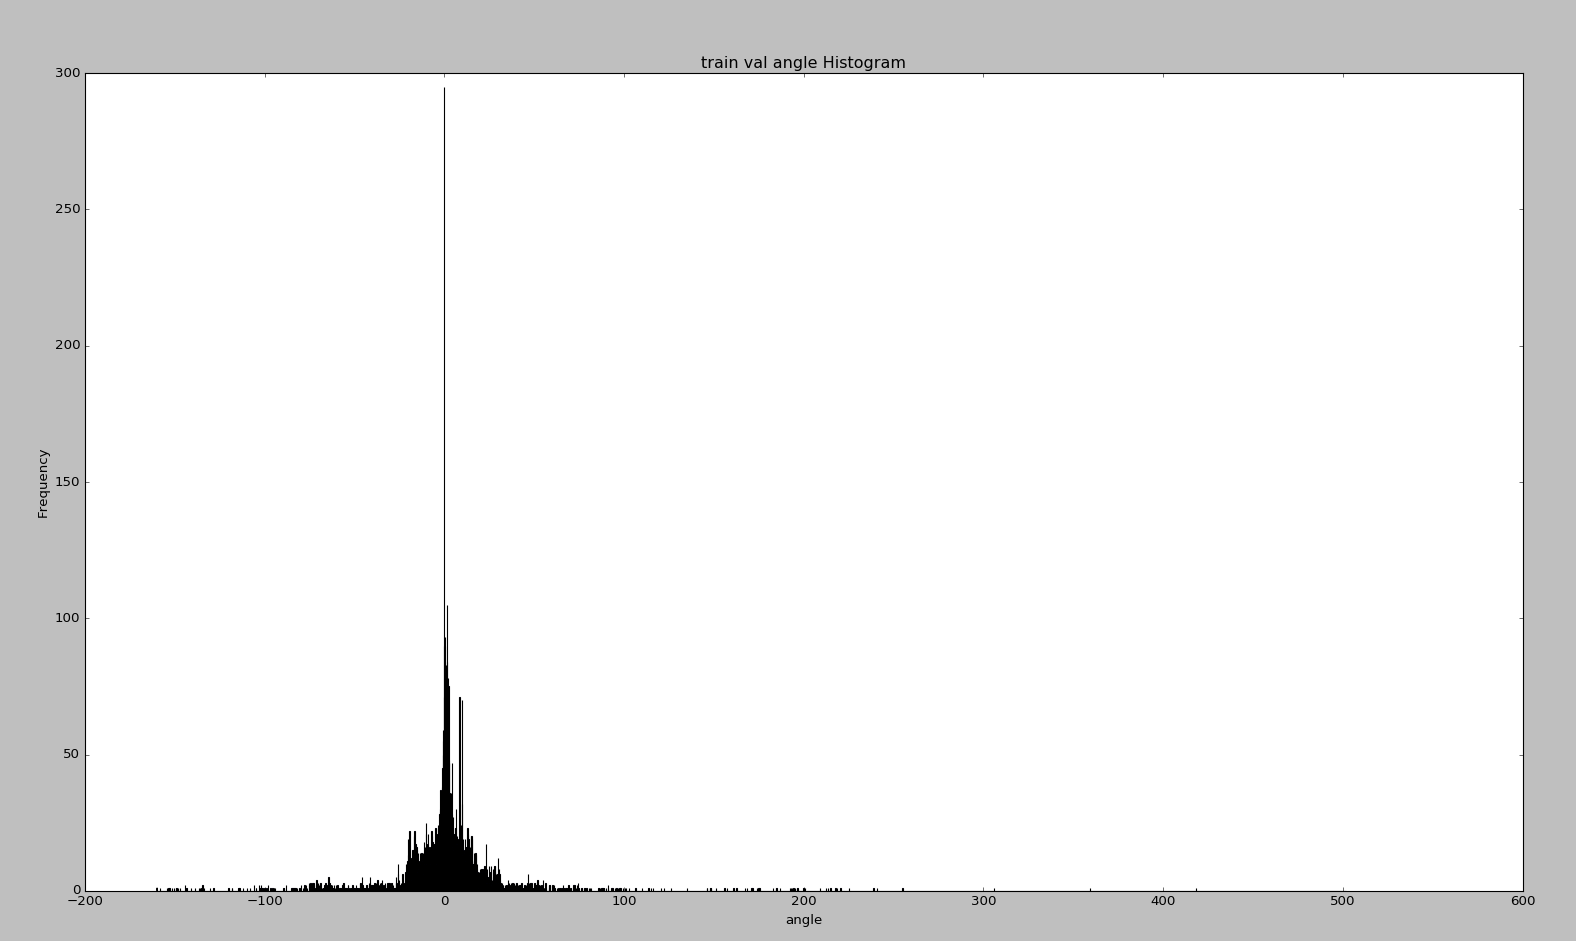
\includegraphics[width=0.8\linewidth]{fig4.png}
	\end{center}
	\caption{Distribution of all the steering angles for driving dataset}
	\label{fig:long4}
\end{figure}

\begin{figure}[h]
	\begin{center}		
		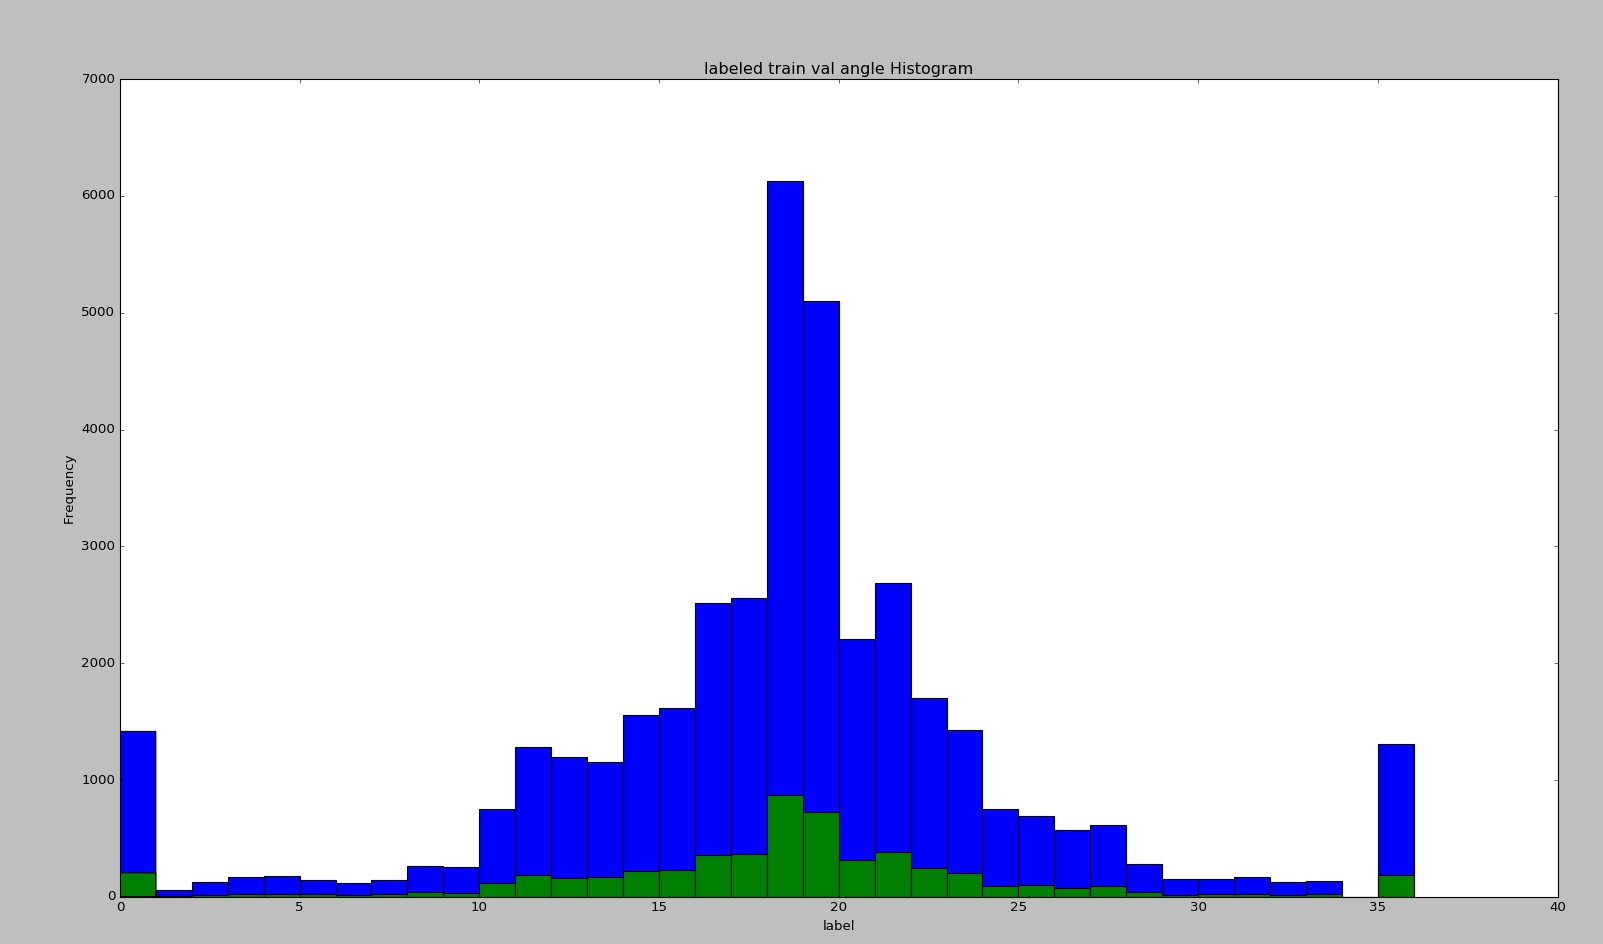
\includegraphics[width=0.8\linewidth]{fig3.png}
	\end{center}
	\caption{Distribution of training and testing labels}
	\label{fig:long3}
\end{figure}




\section{Experiment}

\subsection{Design training process}

\subsubsection{Solver}
In the Caffe framework, the training process is pre-state in solver file. The solver orchestrates model optimization by coordinating the network’s forward inference and backward gradients to form parameter updates that attempt to improve the loss. The responsibilities of learning are divided between the Solver for overseeing the optimization and generating parameter updates and the Net for yielding loss and gradients.\par


The solver
\begin{itemize}
	\item scaffolds the optimization bookkeeping and creates the training network for learning and test network(s) for evaluation.
	\item iteratively optimizes by calling forward / backward and updating parameters
	\item (periodically) evaluates the test networks
	\item snapshots the model and solver state throughout the optimization
\end{itemize}

Where each iteration
\begin{itemize}
	\item calls network forward to compute the output and loss
	\item calls network backward to compute the gradients
	\item incorporates the gradients into parameter updates according to the solver method
	\item updates the solver state according to learning rate, history, and method
\end{itemize}

\subsection{Stochastic Gradient Descent}

Stochastic gradient descent (type: "SGD") updates the weights $W$ by a linear combination of the negative gradient $\nabla L(W)$ and the previous weight update $V_t$. The learning rate α is the weight of the negative gradient. The momentum $μ$ is the weight of the previous update.\par

Formally, we have the following formulas to compute the update value $V_{t+1}$
and the updated weights $W_{t+1}$ at iteration $t+1$, given the previous weight update $V_t$ and current weights $W_{t}$:
\[V_{t+1} = μV_{t} - α\nabla L(W_{t})  \]
\[W_{t+1} = W_{t} + V_{t+1}  \]


\begin{figure}[h]
	\begin{center}
		
		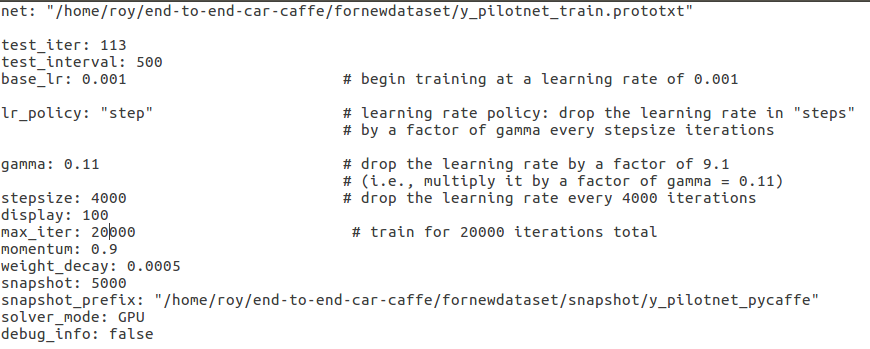
\includegraphics[width=0.8\linewidth]{fig6.png}
	\end{center}
	\caption{The solver definition}
	\label{fig:long6}
\end{figure}





\section{Result analysis}


\subsection{Training process}

We can tell from the figure that, when iteration goes from 0 to 5,000, train loss decreases rapidly from 3.6 to 1.4, and test accuracy increases rapidly from 0.06 to 0.6. Then when iteration goes from 5,000 to 20,000, train loss decreases slightly from 1.4 to 1.3, and test accuracy increases slightly from 0.6 to 0.7. Since the train loss converge from 3.6 to 1.4, it seems that Pilotnet is trying to classify the driving dataset, but train loss diverts between 0.6 and 1.5 after 5,000 iterations, it seems that the trained model can performance quite well on some of the data and performance quite bad on some other data.


\begin{figure}[h]
	\begin{center}
		
		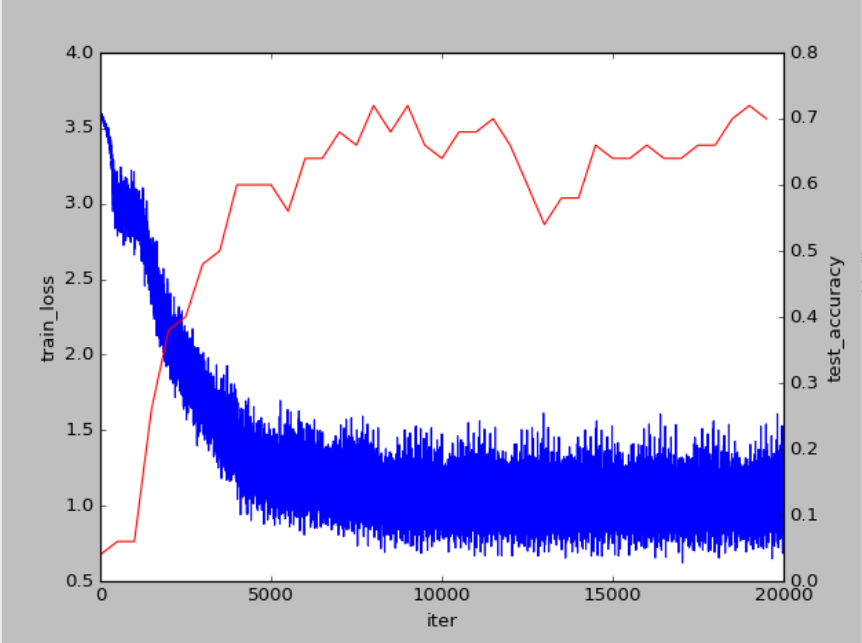
\includegraphics[width=0.8\linewidth]{fig5.png}
	\end{center}
	\caption{The train loss and test accuracy for 20000 iterations}
	\label{fig:long5}
\end{figure}




\subsection{Testing process}
The test accuracy is generated by the embedded program of Caffe framework, since I set the batch size for test is 50, so each time Caffe compute the test accuracy, it will always choose the first 50 images in the testing dataset and use them as input for the trained Pilotnet and generate the accuracy out of these 50 images.\par  

So I write a Python script to compute the accuracy for all the testing dataset, and called the predict result which is the same as the ground truth a match label.\par

\begin{figure}[h]
	\begin{center}
		
		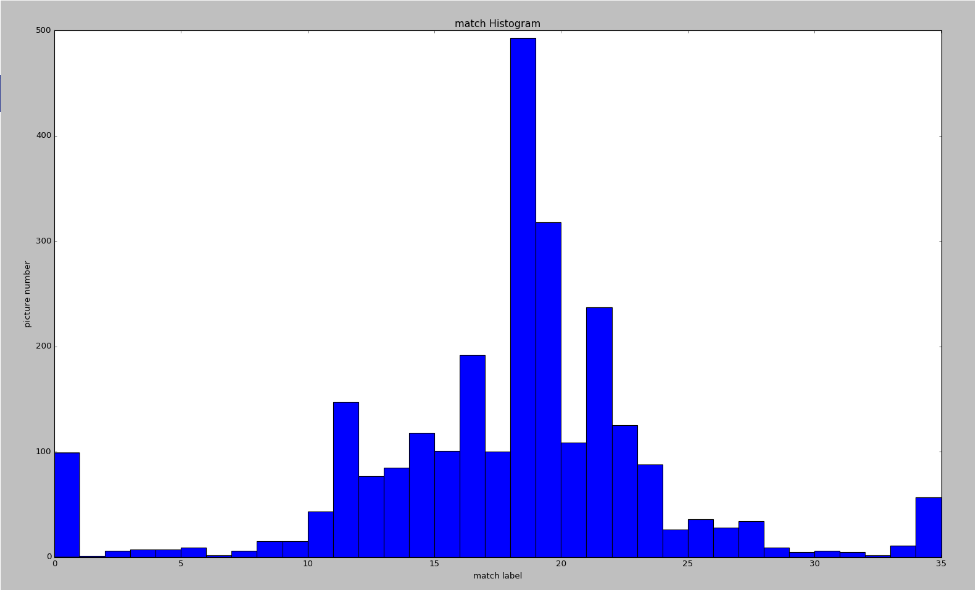
\includegraphics[width=0.8\linewidth]{fig7.png}
	\end{center}
	\caption{The distribution of matched label}
	\label{fig:long7}
\end{figure}


I use L2 loss function to estimate the performance of the trained Pilotnet. L2 Loss Function is the sum of the all the squared differences between the true value and the predicted value.
\[L2LossFunction = \Sigma_{i = 1}^{n}(y_{true}-y_{predicted})^2   \]

\begin{figure}[ht]
	\centering
	\begin{subfigure}[b]{0.21\textwidth}
		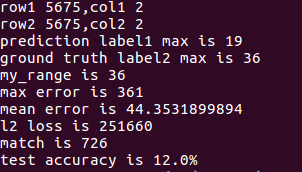
\includegraphics[width=\textwidth]{fig9.png}
		\caption{Test result for model that has been trained 22 iterations}
		\label{fig:acc1}
	\end{subfigure}
	\begin{subfigure}[b]{0.25\textwidth}
		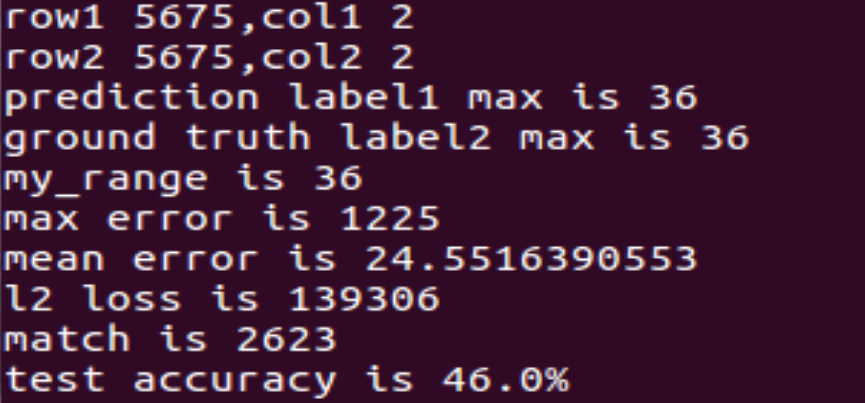
\includegraphics[width=\textwidth]{fig8.png}
		\caption{Test result for model that has been trained 20,000 iterations}
		\label{fig:acc2}
	\end{subfigure}
	\caption{The compare result between a heavily trained model and a barely trained model}
	\label{fig:tworesult}
\end{figure}

The $max error$ means the max prediction error in all the testing data. The $mean error$ means the average error for all the testing data. The $test accuracy$ is compute from the matched label number over the total testing label number.

\section{Conclusion}
\begin{itemize}
	\item For the driving dataset that captured in the real world, Pilotnet has the ability to predict the steering angle when the input is only the image.
	\item Using SGD optimization method for back-propagation in the training process can make the training loss converge.
	\item The distribution of labels for the training dataset will influence the trained model and the testing result.
	
\end{itemize}

\section{Future work}
\begin{itemize}
	\item For the driving dataset that captured in the real world, I should collect more data that captured under different weather situations. Besides, I could apply data augmentation method like crop and adding noise for the original dataset.
	\item Using SGD optimization method for back-propagation in the training process can make the training loss converge, but Adam optimization method is a more popular optimization method, it may have better performance for converge the training loss.
	\item It is true that the Pilotnet can predict the steering angle for input driving image, but it is first mentioned in a paper that published in 2016, maybe we can modify the Pilotnet to have better performance for the same purpose.
	
\end{itemize}


\begin{thebibliography}{00}
\bibitem{b1} Mariusz Bojarski, Davide Del Testa, Daniel Dworakowski, Bernhard Firner, Beat Flepp, Prasoon Goyal, Lawrence D. Jackel, Mathew Monfort, Urs Muller, Jiakai Zhang, Xin Zhang, Jake Zhao, Karol Zieba  ``End to End Learning for Self-Driving Cars'' 
\bibitem{b2} $https://www.quora.com/What-does-end-to-end-mean-in-deep-learning-methods$
\bibitem{b3} $https://github.com/SullyChen$
\bibitem{b4} $http://caffe.berkeleyvision.org$/
\bibitem{b5} $https://en.wikipedia.org/wiki/Convolutional_neural_network$
\end{thebibliography}


\end{document}
